\documentclass{article}

\usepackage[T1]{fontenc}
\usepackage[polish]{babel}
\usepackage[utf8]{inputenc}
\usepackage{graphicx}
\usepackage{subcaption} 
\usepackage[margin=2cm]{geometry}
\usepackage{listings}
\usepackage{color}
\usepackage{amsmath}
\usepackage{tcolorbox}
\usepackage{systeme}
\usepackage{indentfirst}

\definecolor{red}{RGB}{245, 63, 60}
\definecolor{blue}{RGB}{59, 69, 245}
\definecolor{green}{RGB}{59, 245, 117}
\definecolor{yellow}{RGB}{245, 207, 59}

\title{Raport Zadanie NUM5}
\date{02.12.2023}
\author{Tomasz Dziób}

\begin{document}
  \maketitle
  \newpage
  \section{Wstęp techniczny}
  Poniższy raport dotyczy zadania numerycznego NUM5 z listy 4. Załączony program o nazwie \textit{num5.cpp} został napisany w języku \textit{C++}, prezentuje on rozwiązanie oraz korzysta z bibioteki \textit{GNU Plot} w celu stworzenia wykresu. do sprawdzenia obliczeń został użyty plik \textit{check.cpp} również napisany w języku \textit{C++} z wykorzystaniem bibioteki \textit{GSL}. Przed skompilowaniem programu należy zainstalować powyższe biblioteki.

    \subsection{Jak uruchomić program?}
    Razem z załączonymi plikami znajdziemy \textit{Makefile} który służy do uruchomienia programu \textit{num4.cpp} oraz \textit{check.cpp} komendą: \textit{make run}\\

  \section{Nakreślenie problemu}
  Do rozwiązania zadanego problemu zostały wykorzystane metody iteracyjne. Służą one do odnalezienia jak najdokładniejszego przybliżenia wyniku poprzez ciągłe powtarzanie obliczeń do osiągnięcia pewnej, ustalonej dokładności.
  
  Teorytycznie osiągnięcie \textit{dokładnego wyniku} jest możliwe gdy ilość wykonanych iteracji dąży do nieskończoności, praktycznie zadowalający wynik można uzyskać już po kilkunastu powtórzeniach (warto zaznaczyć, że typ danych wejściowych głównie uzależnia ilość iteracji).

  
  Podczas rozwiązywania równań typu \textbf{Ay = b} istota metod iteracyjnych bazuje na rozkładzie macierzy \textit{A} na sumę dwóch macierzy \textbf{$A_1$} oraz \textbf{$A_2$}.

  \begin{center}
    \large Ay = b \qquad \qquad \qquad $A = A_1 + A_2$ \\
    \raisebox{-0.1cm}{\large  $(A_1 + A_2)x = b$} \\
    \raisebox{-0.35cm}{\large  $A_1x = b - A_2x$}
  \end{center}

  Z tego uzyskujemy wzór ogólny na kolejną iterację:

  \begin{center}
    \large  $A_1x^{k+1} = b - A_2x^{k}$
  \end{center}

  W metodach iteracyjnych macierz \textit{A} możemy zapisać w postaci \textit{A = \textcolor{blue}{L} + \textcolor{red}{D} + \textcolor{green}{U}}. Gdzie L to macierz trójkątna dolna \underline{bez diagonali}, U to macierz trójkątna górna \underline{bez diagonali} a D to sama diagonala.
  \begin{center}
    $\begin{bmatrix}
      \textcolor{red}{\bullet} & \textcolor{green}{\bullet} & \textcolor{green}{\bullet} & \textcolor{green}{\bullet} & \textcolor{green}{\bullet} \\
      \textcolor{blue}{\bullet} & \textcolor{red}{\bullet} & \textcolor{green}{\bullet} & \textcolor{green}{\bullet} & \textcolor{green}{\bullet} \\
      \textcolor{blue}{\bullet} & \ddots & \ddots & \ddots & \textcolor{green}{\bullet} \\
      \textcolor{blue}{\bullet} & \textcolor{blue}{\bullet} & \textcolor{blue}{\bullet} & \textcolor{red}{\bullet} & \textcolor{green}{\bullet} \\
      \textcolor{blue}{\bullet} & \textcolor{blue}{\bullet} & \textcolor{blue}{\bullet} & \textcolor{blue}{\bullet} & \textcolor{red}{\bullet} \\
    \end{bmatrix}$
  \end{center}
    
  \section{Użyta metoda}
  W zadaniu zostajemy poproszeni o przeanalizowanie dwóch metod, \textit{Jacobiego} oraz \textit{Gaussa-Seidela}.
  \subsection{Wyprowadzanie wzorów}
  Dla metody \textbf{Jacobiego} macierze $A_1$ oraz $A_2$ przyjmują postać:

  \begin{center}
    \large  $A_1$ = D, \qquad \qquad $A_2$ = L + U
  \end{center}

  Wstawiając do wzoru ogólnego a następnie przechodząc na zapis indeksowy.

  \begin{center}
    \large  $Dx^{k+1} = b - (L+U)x^{k}$ \\
    \raisebox{-0.5cm}{\large  $a_{ii} x_{i}^{k+1} = b_i - \sum\limits_{j \neq i}^{} a_{ij} x_{j}^{k}$} \\
    \raisebox{-1cm}{\Large \textcolor{red}{$x_{i}^{k+1} = \frac{b_i - \sum\limits_{j \neq i}^{} a_{ij} x_{j}^{k}}{a_{ii}}$}} \\

  \end{center}

  Dla metody \textbf{Gaussa-Seidela} macierze $A_1$ oraz $A_2$ przyjmują postać:

  \begin{center}
    \large  $A_1$ = D + L, \qquad \qquad $A_2$ = U
  \end{center}

  Wstawiając do wzoru ogólnego a następnie przechodząc na zapis indeksowy.

  \begin{center}
    \large  $(D+L)x^{k+1} = b - Ux^{k}$ \\
    \raisebox{-0.5cm}{\large  $\sum\limits_{j \leq i}^{} a_{ij} x_{j}^{k+1} = b_i - \sum\limits_{j > i}^{} a_{ij} x_{j}^{k}$}
    \begin{flushleft}
      \normalsize Sumę przy $x_{j}^{k+1}$ można rozpisać na diagonalę oraz macierz wstęgi pod nią:
    \end{flushleft}
    \raisebox{-0.1cm}{\large $\sum\limits_{j < i}^{} a_{ij} x_{j}^{k+1} + a_{ii} x_{i}^{k+1} = b_i - \sum\limits_{j > i}^{} a_{ij} x_{j}^{k}$} \\
    \raisebox{-1cm}{\Large \textcolor{red}{$ x_{i}^{k+1} = \frac{b_i - \sum\limits_{j < i}^{} a_{ij} x_{j}^{k+1} - \sum\limits_{j > i}^{} a_{ij} x_{j}^{k}}{a_{ii}}$}} \\
  \end{center}

  Po powyższych przekształceniach otrzymaliśmy wzory do zastosowania na maszynie cyfrowej. We wzorze na metodę \textit{Gaussa-Seidela} jedyną niepokojąca rzeczą może być występowanie $x_{j}^{k+1}$ w jednej z sum, nie należy się jednak tym przejmować ponieważ ten element zawsze jest już wyliczony.
  \subsection{Zastosowanie w zadaniu}
  W zadaniu mamy zastosować powyższe metody do zadanego układu równań:
  \begin{center}
  $\begin{bmatrix}
    3 & 1 & 0.15 &  &  \\
    1 & 3 & 1 & \ddots &  \\
    0.15 & \ddots & \ddots & \ddots & 0.15 \\
     & \ddots & 1 & 3 & 1 \\
     &  & 0.15 & 1 & 3 \\
  \end{bmatrix}$
  $x=$ 
  $\begin{bmatrix}
    1 \\
    2 \\
    3 \\
    \vdots \\
    N-1 \\
    N \\
  \end{bmatrix}$
  \end{center}
  Uwzględniając strukturę macierzy, sumy występujące w powyższych wzorach da się uprościć do kilku operacji. Pozwala to na unikanie mnożenia przez zero oraz zmniejsza złożoność algorytmu.
  
  \section{Uzyskany wynik}
  Obliczenia wykonane z użyciem metody \textit{Jacobiego} pokrywa się z wynikiem uzyskanym metodą \textit{Gaussa-Seidela} oraz z pojedynczego wywołania komendy \textit{solve} w bibiotece \textit{GSL}.
  \newpage
    \begin{flushleft}
      $\bullet$ Wynik obliczony przez program \textit{num5.cpp} \\
      \raisebox{-0.25cm}{\qquad $\circ$ \textbf{Metoda Jacobiego}}
    \end{flushleft}

    \begin{center}
      \begin{tcolorbox}
        Wektor x:\\ 
        0.178015 0.381162 0.565284 0.754771 0.94342 1.13206 1.32076 1.50943 1.69811 1.88679 2.07547 2.26415 2.45283 2.64151 2.83019 3.01887 3.20755 3.39623 3.58491 3.77358 3.96226 4.15094 4.33962 4.5283 4.71698 4.90566 5.09434 5.28302 5.4717 5.66038 5.84906 6.03774 6.22642 6.41509 6.60377 6.79245 6.98113 7.16981 7.35849 7.54717 7.73585 7.92453 8.11321 8.30189 8.49057 8.67925 8.86792 9.0566 9.24528 9.43396 9.62264 9.81132 10 10.1887 10.3774 10.566 10.7547 10.9434 11.1321 11.3208 11.5094 11.6981 11.8868 12.0755 12.2642 12.4528 12.6415 12.8302 13.0189 13.2075 13.3962 13.5849 13.7736 13.9623 14.1509 14.3396 14.5283 14.717 14.9057 15.0943 15.283 15.4717 15.6604 15.8491 16.0377 16.2264 16.4151 16.6038 16.7925 16.9811 17.1698 17.3585 17.5472 17.7358 17.9245 18.1132 18.3019 18.4906 18.6792 18.8679 19.0566 19.2453 19.434 19.6226 19.8113 20 20.1887 20.3774 20.566 20.7547 20.9434 21.1321 21.3208 21.5094 21.6981 21.8869 22.0754 22.2631 22.4603 22.6134 22.8752 23.2329 21.0616 33.1512\\
        Liczba iteracji: 90
      \end{tcolorbox}

      \begin{flushleft}
        \raisebox{-0.25cm}{\qquad $\circ$ \textbf{Metoda Gaussa-Seidela}}
      \end{flushleft}

        \begin{tcolorbox}
          Wektor x:\\
          0.178015 0.381162 0.565284 0.754771 0.94342 1.13206 1.32076 1.50943 1.69811 1.88679 2.07547 2.26415 2.45283 2.64151 2.83019 3.01887 3.20755 3.39623 3.58491 3.77358 3.96226 4.15094 4.33962 4.5283 4.71698 4.90566 5.09434 5.28302 5.4717 5.66038 5.84906 6.03774 6.22642 6.41509 6.60377 6.79245 6.98113 7.16981 7.35849 7.54717 7.73585 7.92453 8.11321 8.30189 8.49057 8.67925 8.86792 9.0566 9.24528 9.43396 9.62264 9.81132 10 10.1887 10.3774 10.566 10.7547 10.9434 11.1321 11.3208 11.5094 11.6981 11.8868 12.0755 12.2642 12.4528 12.6415 12.8302 13.0189 13.2075 13.3962 13.5849 13.7736 13.9623 14.1509 14.3396 14.5283 14.717 14.9057 15.0943 15.283 15.4717 15.6604 15.8491 16.0377 16.2264 16.4151 16.6038 16.7925 16.9811 17.1698 17.3585 17.5472 17.7358 17.9245 18.1132 18.3019 18.4906 18.6792 18.8679 19.0566 19.2453 19.434 19.6226 19.8113 20 20.1887 20.3774 20.566 20.7547 20.9434 21.1321 21.3208 21.5094 21.6981 21.8869 22.0754 22.2631 22.4603 22.6134 22.8752 23.2329 21.0616 33.1512\\
          Liczba iteracji: 19
        \end{tcolorbox}


      \begin{flushleft}
        $\bullet$ Wynik obliczony przez program \textit{check.cpp}
      \end{flushleft}

      \begin{tcolorbox}
        Wektor x:\\
        0.178015 0.381162 0.565284 0.754771 0.94342 1.13206 1.32076 1.50943 1.69811 1.88679 2.07547 2.26415 2.45283 2.64151 2.83019 3.01887 3.20755 3.39623 3.58491 3.77358 3.96226 4.15094 4.33962 4.5283 4.71698 4.90566 5.09434 5.28302 5.4717 5.66038 5.84906 6.03774 6.22642 6.41509 6.60377 6.79245 6.98113 7.16981 7.35849 7.54717 7.73585 7.92453 8.11321 8.30189 8.49057 8.67925 8.86792 9.0566 9.24528 9.43396 9.62264 9.81132 10 10.1887 10.3774 10.566 10.7547 10.9434 11.1321 11.3208 11.5094 11.6981 11.8868 12.0755 12.2642 12.4528 12.6415 12.8302 13.0189 13.2075 13.3962 13.5849 13.7736 13.9623 14.1509 14.3396 14.5283 14.717 14.9057 15.0943 15.283 15.4717 15.6604 15.8491 16.0377 16.2264 16.4151 16.6038 16.7925 16.9811 17.1698 17.3585 17.5472 17.7358 17.9245 18.1132 18.3019 18.4906 18.6792 18.8679 19.0566 19.2453 19.434 19.6226 19.8113 20 20.1887 20.3774 20.566 20.7547 20.9434 21.1321 21.3208 21.5094 21.6981 21.8869 22.0754 22.2631 22.4603 22.6134 22.8752 23.2329 21.0616 33.1512 
      \end{tcolorbox}
    \end{center}

    Wszystkie wyniki wyglądają identycznie z racji uciętych wartości. Dokładność została ustalona na $1 \cdot e^{-8}$. Oznacza to, że błąd numeryczny wkrada się dopiero po 8 miejscu po przecinku. Jest to wystarczająca dokładność dla wyników tego rzędu.

    jesteśmy wstanie zaobserowować znaczną różnicę jeśli chodzi o liczbę wykonanych iteracji w obu metodach. Szybsza okazuje się metoda \textit{Gaussa-Seidela} która już 19 powtórzeniach dała pożądany wynik.
    \begin{figure}[!ht]
      \centering
      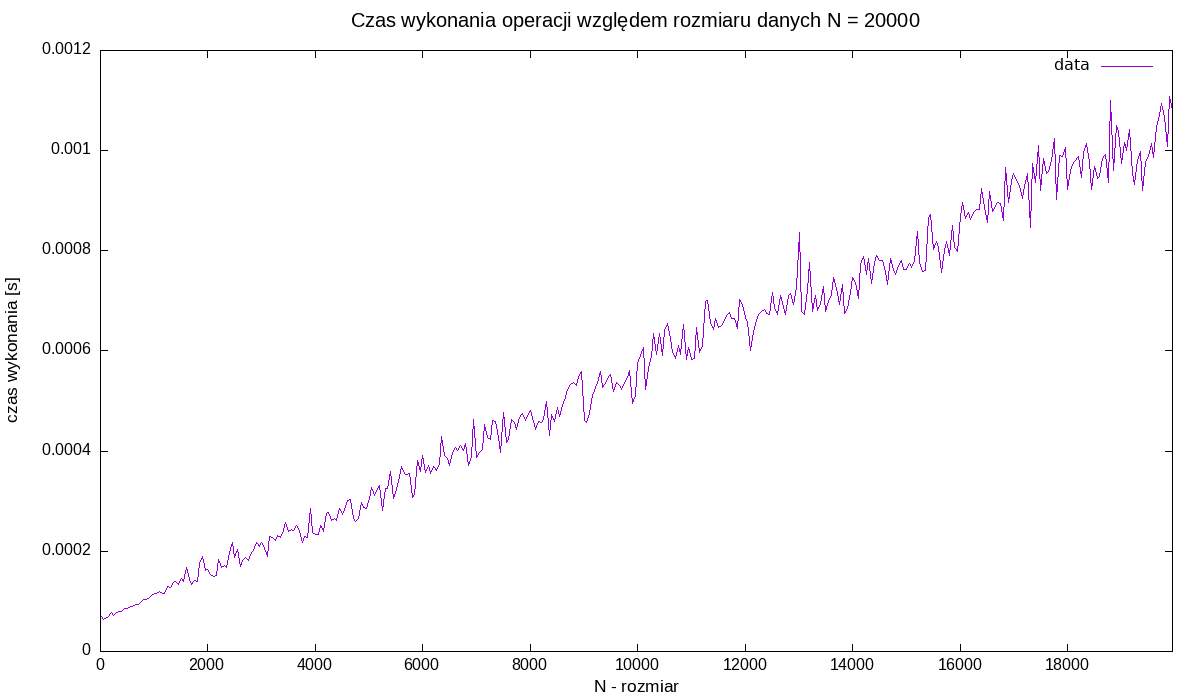
\includegraphics[width=1.0\linewidth]{wyniki.eps}
      \caption{Wynik uzyskany po uruchomienu programu \textit{num5.cpp}}
    \end{figure}
  \newpage
  Przedstawiając ten wynik na wykresie wyglądałoby to tak jak powyżej. Wartośc błędu bezwględnego to \\ $|x^k - x^{k-1}|$ wyświetlane na wykresie w skali logarytmicznej.


  \section{Podsumowanie}
  Metody iteracyjne błyszczą najbardziej gdy nie potrzebujemy pełnej dokładności rozwiązania. Jeśli wystarcza nam przybliżone rozwiązanie, metody iteracyjne mogą być bardziej efektywne, ponieważ mogą zatrzymać się po osiągnięciu pewnego akceptowalnego poziomu dokładności, co może przyspieszyć obliczenia.
  
  Co więcej są one często bardziej efektywne dla dużych, rzadkich macierzy, gdzie większość elementów jest równa zero. Faktoryzacje, na przykład LU, może prowadzić do dużej liczby operacji na zerowych elementach, co jest marnotrawstwem zasobów.

  Złożoność obliczeniowa dla macierzy gęstej wykorzystując faktoryzację to $O(N^3)$ podczas gdy używając metody iteracyjnej uzyskamy wynik zależny od \textit{k} iteracji czyli $O(k \cdot N^2)$.
\end{document}